%%%% Paramétrage du cours %%%%
\def\xxactivite{\ifprof TP -- Corrigé  \else  TP \fi}
\def\xxauteur{\textsl{Xavier Pessoles}}

%\fichefalse
%\proftrue
%\tdfalse
%\courstrue

% Déclaration des titres
% -------------------------------------


\graphicspath{{../../style/png/}{images/}{../../exos//}}
\lstinputpath{{../../exos//}}

\def\discipline{Informatique}
\def\xxtete{Informatique}

\def\classe{\textsf{MPSI}}
\def\xxnumpartie{1}
\def\xxpartie{Architecture matérielle et initiation à l'algorithmique}
\def\xxdate{11 Décembre 2019}

\def\xxchapitre{08}
\def\xxnumchapitre{08}
\def\xxnomchapitre{Représentation des nombres}
\def\xxnumactivite{08}

\def\xxposongletx{2}
\def\xxposonglettext{1.45}
\def\xxposonglety{19}%16

\def\xxonglet{\textsf{Cycle 01}}
\def\xxauteur{\textsl{Émilien Durif -- Sylvaine Kleim \\ Xavier Pessoles }}


\def\xxpied{%
Cycle \xxnumpartie -- \xxpartie\\
Chapitre \xxnumchapitre -- \xxactivite -\xxnumactivite -- \xxnomchapitre%
}

\setcounter{secnumdepth}{5}
\chapterimage{Fond_ALG}
\def\xxfigures{}

\def\xxcompetences{%
\textsl{%
%\vspace{-.5cm}
\textbf{Savoirs et compétences :}\\
\vspace{-.1cm}
\begin{itemize}[label=\ding{112},font=\color{ocre}]
\item AA.C2 : Appréhender les limitations intrinsèques à la manipulation informatique des nombres
\item AA.C3 : Initier un sens critique au sujet de la qualité et de la précision des résultats de calculs numériques sur ordinateur
\item AA.S4 : Principe de la représentation des nombres entiers en mémoire
\item AA.S5 : Principe de la représentation des nombres réels en mémoire
\end{itemize}
}}


%Infos sur les supports
\def\xxtitreexo{Représentation des nombres}
\def\xxsourceexo{\hspace{.2cm} \footnotesize{
}}
%\def\xxtitreexo{Titre EXO}
%\def\xxsourceexo{\hspace{.2cm} \footnotesize{Source EXO}}


%---------------------------------------------------------------------------





\def\xxfigures{
%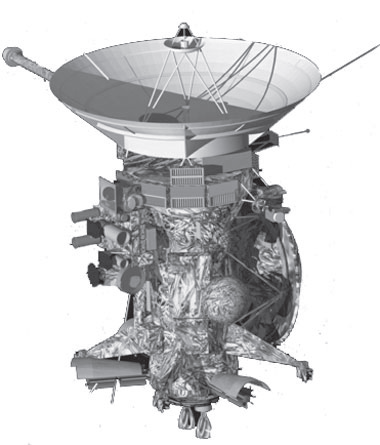
\includegraphics[width=.6\linewidth]{fig_00}
}%figues de la page de garde


\iflivret
\pagestyle{empty}


%%%%%%%% PAGE DE GARDE COURS
\ifcours
% ==== BANDEAU DES TITRES ==== 
\begin{tikzpicture}[remember picture,overlay]
\node at (current page.north west)
{\begin{tikzpicture}[remember picture,overlay]
\node[anchor=north west,inner sep=0pt] at (0,0) {\includegraphics[width=\paperwidth]{\thechapterimage}};
\draw[anchor=west] (-2cm,-8cm) node [line width=2pt,rounded corners=15pt,draw=ocre,fill=white,fill opacity=0.6,inner sep=40pt]{\strut\makebox[22cm]{}};
\draw[anchor=west] (1cm,-8cm) node {\huge\sffamily\bfseries\color{black} %
\begin{minipage}{1cm}
\rotatebox{90}{\LARGE\sffamily\textsc{\color{ocre}\textbf{\xxnumpartie}}}
\end{minipage} \hfill
\begin{minipage}[c]{14cm}
\begin{titrepartie}
\begin{flushright}
\renewcommand{\baselinestretch}{1.1} 
\Large\sffamily\textsc{\textbf{\xxpartie}}
\renewcommand{\baselinestretch}{1} 
\end{flushright}
\end{titrepartie}
\end{minipage} \hfill
\begin{minipage}[c]{3.5cm}
{\large\sffamily\textsc{\textbf{\color{ocre} \discipline}}}
\end{minipage} 
 };
\end{tikzpicture}};
\end{tikzpicture}
% ==== FIN BANDEAU DES TITRES ==== 


% ==== ONGLET 
\begin{tikzpicture}[overlay]
\node[shape=rectangle, 
      rounded corners = .25 cm,
	  draw= ocre,
	  line width=2pt, 
	  fill = ocre!10,
	  minimum width  = 2.5cm,
	  minimum height = 3cm,] at (18.3cm,0) {};
\node at (17.7cm,0) {\rotatebox{90}{\textbf{\Large\color{ocre}{\classe}}}};
%{};
\end{tikzpicture}
% ==== FIN ONGLET 


\vspace{3.5cm}

\begin{tikzpicture}[remember picture,overlay]
\draw[anchor=west] (-2cm,-6cm) node {\huge\sffamily\bfseries\color{black} %
\begin{minipage}{2cm}
\begin{center}
\LARGE\sffamily\textsc{\color{ocre}\textbf{\xxactivite}}
\end{center}
\end{minipage} \hfill
\begin{minipage}[c]{15cm}
\begin{titrechapitre}
\renewcommand{\baselinestretch}{1.1} 
%\Large\sffamily\textsc{\textbf{\xxnumchapitre}}
%
%\Large\sffamily\textsc{\textbf{\xxchapitre}}
\vspace{.5cm}

\renewcommand{\baselinestretch}{1} 
\normalsize\normalfont
\xxcompetences
\end{titrechapitre}
\end{minipage}  };
\end{tikzpicture}
\vfill

\begin{flushright}
\begin{minipage}[c]{.3\linewidth}
\begin{center}
\xxfigures
\end{center}
\end{minipage}\hfill
\begin{minipage}[c]{.6\linewidth}
\startcontents
%\printcontents{}{1}{}
\printcontents{}{1}{}
\end{minipage}
\end{flushright}

\begin{tikzpicture}[remember picture,overlay]
\draw[anchor=west] (4.5cm,-.7cm) node {
\begin{minipage}[c]{.2\linewidth}
\begin{flushright}

\includegraphics[width=2cm]{logoCC}
\end{flushright}
\end{minipage}
\begin{minipage}[c]{.2\linewidth}
\textsl{\xxauteur} \\
\textsl{\classe}
\end{minipage}
 };
\end{tikzpicture}

\newpage
\pagestyle{fancy}

%\newpage
%\pagestyle{fancy}

\else
\fi
%% FIN PAGE DE GARDE DES COURS

%%%%%%%% PAGE DE GARDE TD
\iftd
%\begin{tikzpicture}[remember picture,overlay]
%\node at (current page.north west)
%{\begin{tikzpicture}[remember picture,overlay]
%\draw[anchor=west] (-2cm,-3.25cm) node [line width=2pt,rounded corners=15pt,draw=ocre,fill=white,fill opacity=0.6,inner sep=40pt]{\strut\makebox[22cm]{}};
%\draw[anchor=west] (1cm,-3.25cm) node {\huge\sffamily\bfseries\color{black} %
%\begin{minipage}{1cm}
%\rotatebox{90}{\LARGE\sffamily\textsc{\color{ocre}\textbf{\xxnumpartie}}}
%\end{minipage} \hfill
%\begin{minipage}[c]{13.5cm}
%\begin{titrepartie}
%\begin{flushright}
%\renewcommand{\baselinestretch}{1.1} 
%\Large\sffamily\textsc{\textbf{\xxpartie}}
%\renewcommand{\baselinestretch}{1} 
%\end{flushright}
%\end{titrepartie}
%\end{minipage} \hfill
%\begin{minipage}[c]{3.5cm}
%{\large\sffamily\textsc{\textbf{\color{ocre} \discipline}}}
%\end{minipage} 
% };
%\end{tikzpicture}};
%\end{tikzpicture}

%%%%%%%%%% PAGE DE GARDE TD %%%%%%%%%%%%%%%
%\begin{tikzpicture}[overlay]
%\node[shape=rectangle, 
%      rounded corners = .25 cm,
%	  draw= ocre,
%	  line width=2pt, 
%	  fill = ocre!10,
%	  minimum width  = 2.5cm,
%	  minimum height = 2.5cm,] at (18.5cm,0) {};
%\node at (17.7cm,0) {\rotatebox{90}{\textbf{\Large\color{ocre}{\classe}}}};
%%{};
%\end{tikzpicture}

% PARTIE ET CHAPITRE
%\begin{tikzpicture}[remember picture,overlay]
%\draw[anchor=west] (-1cm,-2.1cm) node {\large\sffamily\bfseries\color{black} %
%\begin{minipage}[c]{15cm}
%\begin{flushleft}
%\xxnumchapitre \\
%\xxchapitre
%\end{flushleft}
%\end{minipage}  };
%\end{tikzpicture}

% BANDEAU EXO
\iflivret % SI LIVRET
\begin{tikzpicture}[remember picture,overlay]
\draw[anchor=west] (-2cm,-3.3cm) node {\huge\sffamily\bfseries\color{black} %
\begin{minipage}{5cm}
\begin{center}
\LARGE\sffamily\color{ocre}\textbf{\textsc{\xxactivite}}

\begin{center}
\xxfigures
\end{center}

\end{center}
\end{minipage} \hfill
\begin{minipage}[c]{12cm}
\begin{titrechapitre}
\renewcommand{\baselinestretch}{1.1} 
\large\sffamily\textbf{\textsc{\xxtitreexo}}

\small\sffamily{\textbf{\textit{\color{black!70}\xxsourceexo}}}
\vspace{.5cm}

\renewcommand{\baselinestretch}{1} 
\normalsize\normalfont
\xxcompetences
\end{titrechapitre}
\end{minipage}};
\end{tikzpicture}
\else % ELSE NOT LIVRET
\begin{tikzpicture}[remember picture,overlay]
\draw[anchor=west] (-2cm,-4.5cm) node {\huge\sffamily\bfseries\color{black} %
\begin{minipage}{5cm}
\begin{center}
\LARGE\sffamily\color{ocre}\textbf{\textsc{\xxactivite}}

\begin{center}
\xxfigures
\end{center}

\end{center}
\end{minipage} \hfill
\begin{minipage}[c]{12cm}
\begin{titrechapitre}
\renewcommand{\baselinestretch}{1.1} 
\large\sffamily\textbf{\textsc{\xxtitreexo}}

\small\sffamily{\textbf{\textit{\color{black!70}\xxsourceexo}}}
\vspace{.5cm}

\renewcommand{\baselinestretch}{1} 
\normalsize\normalfont
\xxcompetences
\end{titrechapitre}
\end{minipage}};
\end{tikzpicture}

\fi

\else   % FIN IF TD
\fi


%%%%%%%% PAGE DE GARDE FICHE
\iffiche
\begin{tikzpicture}[remember picture,overlay]
\node at (current page.north west)
{\begin{tikzpicture}[remember picture,overlay]
\draw[anchor=west] (-2cm,-2.25cm) node [line width=2pt,rounded corners=15pt,draw=ocre,fill=white,fill opacity=0.6,inner sep=40pt]{\strut\makebox[22cm]{}};
\draw[anchor=west] (1cm,-2.25cm) node {\huge\sffamily\bfseries\color{black} %
\begin{minipage}{1cm}
\rotatebox{90}{\LARGE\sffamily\textsc{\color{ocre}\textbf{\xxnumpartie}}}
\end{minipage} \hfill
\begin{minipage}[c]{14cm}
\begin{titrepartie}
\begin{flushright}
\renewcommand{\baselinestretch}{1.1} 
\large\sffamily\textsc{\textbf{\xxpartie} \\} 

\vspace{.2cm}

\normalsize\sffamily\textsc{\textbf{\xxnumchapitre -- \xxchapitre}}
\renewcommand{\baselinestretch}{1} 
\end{flushright}
\end{titrepartie}
\end{minipage} \hfill
\begin{minipage}[c]{3.5cm}
{\large\sffamily\textsc{\textbf{\color{ocre} \discipline}}}
\end{minipage} 
 };
\end{tikzpicture}};
\end{tikzpicture}

\iflivret
\begin{tikzpicture}[overlay]
\node[shape=rectangle, 
      rounded corners = .25 cm,
	  draw= ocre,
	  line width=2pt, 
	  fill = ocre!10,
	  minimum width  = 2.5cm,
	  minimum height = 2.5cm,] at (18.5cm,1.1cm) {};
\node at (17.9cm,1.1cm) {\rotatebox{90}{\textsf{\textbf{\large\color{ocre}{\classe}}}}};
%{};
\end{tikzpicture}
\else
\begin{tikzpicture}[overlay]
\node[shape=rectangle, 
      rounded corners = .25 cm,
	  draw= ocre,
	  line width=2pt, 
	  fill = ocre!10,
	  minimum width  = 2.5cm,
%	  minimum height = 2.5cm,] at (18.5cm,1.1cm) {};
	  minimum height = 2.5cm,] at (18.6cm,0cm) {};
\node at (18cm,0cm) {\rotatebox{90}{\textsf{\textbf{\large\color{ocre}{\classe}}}}};
%{};
\end{tikzpicture}

\fi

\else
\fi



\else
\pagestyle{empty}


%%%%%%%% PAGE DE GARDE COURS
\ifcours
% ==== BANDEAU DES TITRES ==== 
\begin{tikzpicture}[remember picture,overlay]
\node at (current page.north west)
{\begin{tikzpicture}[remember picture,overlay]
\node[anchor=north west,inner sep=0pt] at (0,0) {\includegraphics[width=\paperwidth]{\thechapterimage}};
\draw[anchor=west] (-2cm,-8cm) node [line width=2pt,rounded corners=15pt,draw=ocre,fill=white,fill opacity=0.6,inner sep=40pt]{\strut\makebox[22cm]{}};
\draw[anchor=west] (1cm,-8cm) node {\huge\sffamily\bfseries\color{black} %
\begin{minipage}{1cm}
\rotatebox{90}{\LARGE\sffamily\textsc{\color{ocre}\textbf{\xxnumpartie}}}
\end{minipage} \hfill
\begin{minipage}[c]{14cm}
\begin{titrepartie}
\begin{flushright}
\renewcommand{\baselinestretch}{1.1} 
\Large\sffamily\textsc{\textbf{\xxpartie}}
\renewcommand{\baselinestretch}{1} 
\end{flushright}
\end{titrepartie}
\end{minipage} \hfill
\begin{minipage}[c]{3.5cm}
{\large\sffamily\textsc{\textbf{\color{ocre} \discipline}}}
\end{minipage} 
 };
\end{tikzpicture}};
\end{tikzpicture}
% ==== FIN BANDEAU DES TITRES ==== 


% ==== ONGLET 
\begin{tikzpicture}[overlay]
\node[shape=rectangle, 
      rounded corners = .25 cm,
	  draw= ocre,
	  line width=2pt, 
	  fill = ocre!10,
	  minimum width  = 2.5cm,
	  minimum height = 3cm,] at (18.3cm,0) {};
\node at (17.7cm,0) {\rotatebox{90}{\textbf{\Large\color{ocre}{\classe}}}};
%{};
\end{tikzpicture}
% ==== FIN ONGLET 


\vspace{3.5cm}

\begin{tikzpicture}[remember picture,overlay]
\draw[anchor=west] (-2cm,-6cm) node {\huge\sffamily\bfseries\color{black} %
\begin{minipage}{2cm}
\begin{center}
\LARGE\sffamily\textsc{\color{ocre}\textbf{\xxactivite}}
\end{center}
\end{minipage} \hfill
\begin{minipage}[c]{15cm}
\begin{titrechapitre}
\renewcommand{\baselinestretch}{1.1} 
%\Large\sffamily\textsc{\textbf{\xxnumchapitre}}
%
%\Large\sffamily\textsc{\textbf{\xxchapitre}}
\vspace{.5cm}

\renewcommand{\baselinestretch}{1} 
\normalsize\normalfont
\xxcompetences
\end{titrechapitre}
\end{minipage}  };
\end{tikzpicture}
\vfill

\begin{flushright}
\begin{minipage}[c]{.3\linewidth}
\begin{center}
\xxfigures
\end{center}
\end{minipage}\hfill
\begin{minipage}[c]{.6\linewidth}
\startcontents
%\printcontents{}{1}{}
\printcontents{}{1}{}
\end{minipage}
\end{flushright}

\begin{tikzpicture}[remember picture,overlay]
\draw[anchor=west] (4.5cm,-.7cm) node {
\begin{minipage}[c]{.2\linewidth}
\begin{flushright}

\includegraphics[width=2cm]{logoCC}
\end{flushright}
\end{minipage}
\begin{minipage}[c]{.2\linewidth}
\textsl{\xxauteur} \\
\textsl{\classe}
\end{minipage}
 };
\end{tikzpicture}

\newpage
\pagestyle{fancy}

%\newpage
%\pagestyle{fancy}

\else
\fi
%% FIN PAGE DE GARDE DES COURS

%%%%%%%% PAGE DE GARDE TD
\iftd
%\begin{tikzpicture}[remember picture,overlay]
%\node at (current page.north west)
%{\begin{tikzpicture}[remember picture,overlay]
%\draw[anchor=west] (-2cm,-3.25cm) node [line width=2pt,rounded corners=15pt,draw=ocre,fill=white,fill opacity=0.6,inner sep=40pt]{\strut\makebox[22cm]{}};
%\draw[anchor=west] (1cm,-3.25cm) node {\huge\sffamily\bfseries\color{black} %
%\begin{minipage}{1cm}
%\rotatebox{90}{\LARGE\sffamily\textsc{\color{ocre}\textbf{\xxnumpartie}}}
%\end{minipage} \hfill
%\begin{minipage}[c]{13.5cm}
%\begin{titrepartie}
%\begin{flushright}
%\renewcommand{\baselinestretch}{1.1} 
%\Large\sffamily\textsc{\textbf{\xxpartie}}
%\renewcommand{\baselinestretch}{1} 
%\end{flushright}
%\end{titrepartie}
%\end{minipage} \hfill
%\begin{minipage}[c]{3.5cm}
%{\large\sffamily\textsc{\textbf{\color{ocre} \discipline}}}
%\end{minipage} 
% };
%\end{tikzpicture}};
%\end{tikzpicture}

%%%%%%%%%% PAGE DE GARDE TD %%%%%%%%%%%%%%%
%\begin{tikzpicture}[overlay]
%\node[shape=rectangle, 
%      rounded corners = .25 cm,
%	  draw= ocre,
%	  line width=2pt, 
%	  fill = ocre!10,
%	  minimum width  = 2.5cm,
%	  minimum height = 2.5cm,] at (18.5cm,0) {};
%\node at (17.7cm,0) {\rotatebox{90}{\textbf{\Large\color{ocre}{\classe}}}};
%%{};
%\end{tikzpicture}

% PARTIE ET CHAPITRE
%\begin{tikzpicture}[remember picture,overlay]
%\draw[anchor=west] (-1cm,-2.1cm) node {\large\sffamily\bfseries\color{black} %
%\begin{minipage}[c]{15cm}
%\begin{flushleft}
%\xxnumchapitre \\
%\xxchapitre
%\end{flushleft}
%\end{minipage}  };
%\end{tikzpicture}

% BANDEAU EXO
\iflivret % SI LIVRET
\begin{tikzpicture}[remember picture,overlay]
\draw[anchor=west] (-2cm,-3.3cm) node {\huge\sffamily\bfseries\color{black} %
\begin{minipage}{5cm}
\begin{center}
\LARGE\sffamily\color{ocre}\textbf{\textsc{\xxactivite}}

\begin{center}
\xxfigures
\end{center}

\end{center}
\end{minipage} \hfill
\begin{minipage}[c]{12cm}
\begin{titrechapitre}
\renewcommand{\baselinestretch}{1.1} 
\large\sffamily\textbf{\textsc{\xxtitreexo}}

\small\sffamily{\textbf{\textit{\color{black!70}\xxsourceexo}}}
\vspace{.5cm}

\renewcommand{\baselinestretch}{1} 
\normalsize\normalfont
\xxcompetences
\end{titrechapitre}
\end{minipage}};
\end{tikzpicture}
\else % ELSE NOT LIVRET
\begin{tikzpicture}[remember picture,overlay]
\draw[anchor=west] (-2cm,-4.5cm) node {\huge\sffamily\bfseries\color{black} %
\begin{minipage}{5cm}
\begin{center}
\LARGE\sffamily\color{ocre}\textbf{\textsc{\xxactivite}}

\begin{center}
\xxfigures
\end{center}

\end{center}
\end{minipage} \hfill
\begin{minipage}[c]{12cm}
\begin{titrechapitre}
\renewcommand{\baselinestretch}{1.1} 
\large\sffamily\textbf{\textsc{\xxtitreexo}}

\small\sffamily{\textbf{\textit{\color{black!70}\xxsourceexo}}}
\vspace{.5cm}

\renewcommand{\baselinestretch}{1} 
\normalsize\normalfont
\xxcompetences
\end{titrechapitre}
\end{minipage}};
\end{tikzpicture}

\fi

\else   % FIN IF TD
\fi


%%%%%%%% PAGE DE GARDE FICHE
\iffiche
\begin{tikzpicture}[remember picture,overlay]
\node at (current page.north west)
{\begin{tikzpicture}[remember picture,overlay]
\draw[anchor=west] (-2cm,-2.25cm) node [line width=2pt,rounded corners=15pt,draw=ocre,fill=white,fill opacity=0.6,inner sep=40pt]{\strut\makebox[22cm]{}};
\draw[anchor=west] (1cm,-2.25cm) node {\huge\sffamily\bfseries\color{black} %
\begin{minipage}{1cm}
\rotatebox{90}{\LARGE\sffamily\textsc{\color{ocre}\textbf{\xxnumpartie}}}
\end{minipage} \hfill
\begin{minipage}[c]{14cm}
\begin{titrepartie}
\begin{flushright}
\renewcommand{\baselinestretch}{1.1} 
\large\sffamily\textsc{\textbf{\xxpartie} \\} 

\vspace{.2cm}

\normalsize\sffamily\textsc{\textbf{\xxnumchapitre -- \xxchapitre}}
\renewcommand{\baselinestretch}{1} 
\end{flushright}
\end{titrepartie}
\end{minipage} \hfill
\begin{minipage}[c]{3.5cm}
{\large\sffamily\textsc{\textbf{\color{ocre} \discipline}}}
\end{minipage} 
 };
\end{tikzpicture}};
\end{tikzpicture}

\iflivret
\begin{tikzpicture}[overlay]
\node[shape=rectangle, 
      rounded corners = .25 cm,
	  draw= ocre,
	  line width=2pt, 
	  fill = ocre!10,
	  minimum width  = 2.5cm,
	  minimum height = 2.5cm,] at (18.5cm,1.1cm) {};
\node at (17.9cm,1.1cm) {\rotatebox{90}{\textsf{\textbf{\large\color{ocre}{\classe}}}}};
%{};
\end{tikzpicture}
\else
\begin{tikzpicture}[overlay]
\node[shape=rectangle, 
      rounded corners = .25 cm,
	  draw= ocre,
	  line width=2pt, 
	  fill = ocre!10,
	  minimum width  = 2.5cm,
%	  minimum height = 2.5cm,] at (18.5cm,1.1cm) {};
	  minimum height = 2.5cm,] at (18.6cm,0cm) {};
\node at (18cm,0cm) {\rotatebox{90}{\textsf{\textbf{\large\color{ocre}{\classe}}}}};
%{};
\end{tikzpicture}

\fi

\else
\fi



\fi
\setlength{\columnseprule}{.1pt}

\pagestyle{fancy}
\thispagestyle{plain}

\ifprof
\vspace{4.5cm}
\else
\vspace{4.5cm}
\fi

\def\columnseprulecolor{\color{ocre}}
\setlength{\columnseprule}{0.4pt} 

%%%%%%%%%%%%%%%%%%%%%%%

\setcounter{exo}{0}
\vspace{1.5cm}

\begin{multicols}{2}

%\addcontentsline{toc}{subsection}{Exercice 1 -- Opérations sur les polynômes}
\subsection*{Exercice 1 -- Opérations sur les polynômes -- 2.11.3 p.50}
\begin{flushright}
\textit{D'après Frédéric Butin, l'informatique pas à pas en prépa, éditions ellipses.}
\end{flushright}
Un polynôme $P=\sum\limits_{j=0}^{n}a_j X^j \in \mathbb{R}[X]$ de degré $n$ est représenté dans cet exercice par le tableau $P=[a_0,...,a_n]$.

\begin{enumerate}
\item Créer une fonction \texttt{affiche\_poly} qui permet d'afficher un polynôme sous la forme $P=\sum\limits_{j=0}^{n}a_j X^j$.
\item Créer une fonction \texttt{degre\_poly} qui calcule le degré d'un polynôme.
\item Implémenter la somme, le produit et la multiplication par un scalaire comme des fonctions notées \texttt{add\_poly}, \texttt{mul\_poly} et \texttt{mul\_sca\_poly}.
\item Créer une fonction \texttt{prsc\_poly} qui calcule le prduit scalaire canonique de deux polynômes.
\item Créer une fonction \texttt{deriv\_poly} qui calcule la dérivée d'un polynôme.
\end{enumerate}

%\addcontentsline{toc}{subsection}{Exercice 2 -- Produits polynômes}
\subsection*{Exercice 2 -- Produits polynômes -- 2.11.20 p.65}
\begin{flushright}
\textit{D'après Frédéric Butin, l'informatique pas à pas en prépa, éditions ellipses.}
\end{flushright}
Un polynôme $P=\sum\limits_{j=0}^{n}a_j X^j \in \mathbb{R}[X]$ de degré $n$ est représenté dans cet exercice par le tableau $P=[a_0,...,a_n]$.

\begin{enumerate}
\item Créer une fonction \texttt{affiche\_poly} qui permet d'afficher un polynôme sous la forme $P=\sum\limits_{j=0}^{n}a_j X^j$.
\item Créer une fonction \texttt{degre\_poly} qui calcule le degré d'un polynôme.
\item Implémenter le produit de deux polynômes. On notera \texttt{mul\_poly} cette fonction. Donner sa complexité.
\end{enumerate}
On suppose désormais que $n=2^k=2m$. La méthode qui suit permet de calculer le produit de deux polynômes en utilisant le principe <<diviser pour régner>>. 

On pose $P=P_1+X^m P_2$ et $Q=Q_1+X^mQ_2$, où $P_1$ et $Q_1$ sont de degré strictement inférieur à $m$. Ainsi, $PQ=P_1Q_1+X^m\left(P_1Q_2 + Q_1P_2\right)+X^n P_2 Q_2$. 

\begin{enumerate}
\item Calculer le produit de deux polynômes de degré strictement inférieur à $n$ revient donc à calculer 4 produits de deux polynômes de degré inférieur à $\dfrac{n}{2}$. Implémenter cet algorithme en une fonction \texttt{mul\_poly\_div}. Quelle est sa complexité ? Qu'en conclure ?
\item Une autre méthode de calcul consiste à poser $R_1=P_1Q_1$, $R_2=P_2Q_2$ et $R_3=\left(P_1+P_2 \right)\left(Q_1+Q_2 \right)$. Expliciter $PQ$ en fonction des polynômes $R_1$, $R_2$, $R_3$. En déduire un algorithme (appelé algorithme de Karatsuba) permettant le calcul de $PQ$ que l'on implémentera en une fonction \texttt{mul\_poly\_kara}. Comparer la complexité de cet algorithme à celle des algorithmes des questions précédentes. 
\item Que faire quand $n$ n'est pas de la forme $2^k$.
\end{enumerate}


%\addcontentsline{toc}{subsection}{Exercice 3 -- Courbes en polaires}
\subsection*{Exercice 3 -- Courbes en polaires -- 4.6.25 p.111}
\begin{flushright}
\textit{D'après Frédéric Butin, l'informatique pas à pas en prépa, éditions ellipses.}
\end{flushright}

Pour tout $n \in \mathbb{N}^*$, on considère $\Gamma_n$ en coordonnées polaires définie par :
$$
\sigma_n(\theta) = \cos^3 \left( n\theta\right) - \sin^3 \left( n\theta\right).
$$
\begin{enumerate}
\item Représenter la courbe $\Gamma_0$.
\item Représenter sur un même graphique les courbes $\Gamma_j$, pour $j \in \llbracket 0,3\rrbracket $.
\end{enumerate}


%\addcontentsline{toc}{subsection}{Exercice 4 -- Fonction de Takagi}
\subsection*{Exercice 4 -- Fonction de Takagi -- 4.6.26 p.112}
\begin{flushright}
\textit{D'après Frédéric Butin, l'informatique pas à pas en prépa, éditions ellipses.}
\end{flushright}

La fonction de Takagi est définie sur $[0,1]$ par $T:x\mapsto \sum\limits_{k=0}^{\infty} \dfrac{d\left( 2^k x \right)}{2^k}$, où $d(y)$ représente la distance de $y$ à l'entier le plus proche. On peut montrer que cette fonction est continue sur $[0,1]$ mais nulle part dérivable.
\begin{enumerate}
\item Pour tout entier $n\in \mathbb{N}$, majorer $||T-T_n||_{\infty}=\sup\limits_{x\in[0,1]} |T(x)-T_n(x)|$ où $T_n:x \mapsto \sum\limits_{k=0}^{n} \dfrac{d\left( 2^k x \right)}{2^k}$.
\item Représenter le graphe de cette fonction, appelé la courbe du blanc-manger.
\end{enumerate}

%\addcontentsline{toc}{subsection}{Exercice 5 -- Modèle logistique}
\subsection*{Exercice 5 -- Modèle logistique -- 4.6.27 p.113}
\begin{flushright}
\textit{D'après Frédéric Butin, l'informatique pas à pas en prépa, éditions ellipses.}
\end{flushright}

Pour tout $a\in]0,3]$,  on considère la suite récurrente $(u_n)_{n\in\mathbb{N}}$ définie par $u_0 \in \left[ 0,1+\dfrac{1}{a}\right]$ et pour tout $n\in\mathbb{N}^*$, $u_{n+1}=\left(1+a\left(1-u_n \right) \right)u_n$. Cette suite représente, à un facteur près, la population d'une espèce.

\begin{enumerate}
\item Pour $a=1$ et $u_0=0,5$, représenter graphiquement les 10 premiers termes de la suite.
\item On fixe $u_0=0,5$. Créer une procédure qui reçoit en arguments $a_1$, $c$, $a_2$ et permet de représenter les termes $u_n$ pour $n\in \llbracket 100,200 \rrbracket$ et $a=a_1+jc$, $j\in\llbracket 0,\lfloor \dfrac{a_2-a_1}{c}\rfloor \rrbracket$ (les points sont à tracer sont des points de coordonnées $(a,u_n)$.
\item Exécuter cette procédure avec $a_1=2$, $c=0,005$, $a_2=3$ puis avec $a_1=2.84$, $c=0,0001$, $a_2=2,86$.
\end{enumerate}


%\addcontentsline{toc}{subsection}{Exercice 6 -- Enveloppe d'une famille de droites}
\subsection*{Exercice 6 -- Enveloppe d'une famille de droites -- 4.6.28 p.115}
\begin{flushright}
\textit{D'après Frédéric Butin, l'informatique pas à pas en prépa, éditions ellipses.}
\end{flushright}

Doit $\left(D_t\right)_{t\in I}$ une famille de droites du plan affine, où $I$ est un intervalle de $\mathbb{R}$. On munit le plan d'un repère, de sorte que la droite $D_t$ a pour équation :
$$
u(t) x+v(t) y + w(t) = 0.
$$

On suppose que les applications $u$, $v$, $w$ sont de classe $\mathcal{C}^1$ sur $I$ et qu'elles ne s'annulent pas en même temps. 

On cherche une courbe paramétrée $f:I \to \mathbb{R}^2$ telle que pour tout $t\in I$, 
\begin{itemize}
\item $f(t)\in D_t$;
\item $D_t$ est tangente à la courbe en $f(t)$.
\end{itemize}
Quand elle existe, cette courbe est appelée l'enveloppe de la famille de droits $\left(D_t\right)_{t\in I}$. 
\begin{enumerate}
\item On note $f(t)=\left(x(t),y(t)\right)$. Montrer que $\left(x(t),y(t)\right)$ est solution du système :
$$
\left\{
\begin{array}{l}
u(t) x(t) + v(t) y(t)= -w(t) \\
u'(t) x(t) + v'(t) y(t)= -w'(t) \\
\end{array}
\right. .
$$
En déduire qu'au voisinage de tout point $t_0 \in I$ tel que :
$$
\left| 
\begin{array}{cc}
u(t_0) & v(t_0) \\
u'(t_0) & v'(t_0)
\end{array}
\right|
\neq 0
$$,
le système précédent a une unique solution, donnée par :
$$
x(t)=\dfrac{\left| 
\begin{array}{cc}
-w(t) & v(t) \\
-w'(t) & v'(t)
\end{array}
\right|
}{\left| 
\begin{array}{cc}
u(t) & v(t) \\
u'(t) & v'(t)
\end{array}
\right|},
y(t)=\dfrac{\left| 
\begin{array}{cc}
u(t) & -w(t) \\
u'(t) & -w'(t)
\end{array}
\right|
}{\left| 
\begin{array}{cc}
u(t) & v(t) \\
u'(t) & v'(t)
\end{array}
\right|}.
$$
\item Déterminer une paramétrisation de l'enveloppe $E$ de la famille des droites $\left(D_t\right)_{t\in \mathbb{R}}$ d'équation :
$$
\sin(t) x - \cos(t) y -\sin^2(t)=0.
$$
\item Représenter, sur un même graphique, $E$ et plusieurs droites $D_t$.
\end{enumerate}



%\addcontentsline{toc}{subsection}{Exercice 7 -- Hypocycloïde}
\subsection*{Exercice 7 -- Hypocycloïde -- 4.6.29 p.117}
\begin{flushright}
\textit{D'après Frédéric Butin, l'informatique pas à pas en prépa, éditions ellipses.}
\end{flushright}

Un cercle $ \Gamma\left(\Omega,r\right)$ roule sans glisser à l'intérieur du cercle $C\left(O,R\right)$ (où $R>r$). On note $M=M(\theta)$ un point de $\Gamma$ dont étudie la trajectoire. On note $\theta$ l'angle $\left( \widehat{\vect{i},\vect{O\Omega}}\right)$ et $\varphi$ l'angle $\left( \widehat{\vect{\Omega I},\vect{\Omega M}}\right)$. Initialement, $\Omega$ est situé sur l'axe horizontal et $M$ est situé en $I_0$.

\begin{center}
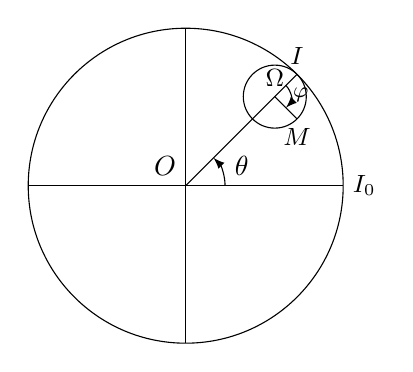
\begin{tikzpicture}
\draw(0,0) circle (2);
\draw({1.6*sqrt(2)/2},{1.6*sqrt(2)/2}) circle (.4);
\draw (-2,0) -- (2,0) node [right] {\small $I_0$};
\draw (0,-2) -- (0,2);
\draw (0,0) node [above left] {$O$} -- ({2*sqrt(2)/2},{2*sqrt(2)/2}) node [above] {\small $I$};
\draw [-latex] (0.5,0) arc (0:45:0.5);
\draw (0.5,0.25) node [right] {$\theta$};
\draw({1.6*sqrt(2)/2},{1.6*sqrt(2)/2}) -- ++ ({.4*sqrt(2)/2},{-.4*sqrt(2)/2}) node [below]{\small $M$};
\draw ({1.6*sqrt(2)/2},{1.6*sqrt(2)/2}) node [above] {\small $\Omega$};
\draw [-latex] ({1.8*sqrt(2)/2},{1.8*sqrt(2)/2}) arc (45:-45:0.2);
\draw (1.24,1.15) node [right] {\footnotesize$\varphi$};
\end{tikzpicture}
\end{center}

\begin{enumerate}
\item Montrer que l'affixe de $M$ est donnée par $z(\theta)=\left(R-r\right) \exp\left(i\theta \right) + r \exp\left(i  m \theta \right)$ où $m=1-\dfrac{R}{r}$. Ainsi, $M$ a pour coordonnées :
$$
\left\{
\begin{array}{l}
x(\theta)= \left(R-r\right) \cos \theta +r \cos \left(m \theta \right) \\
y(\theta)= \left(R-r\right) \sin \theta +r \sin \left(m \theta \right) 
\end{array}
\right. .
$$
\item On choisit $R=4$ et $r=\dfrac{R}{4}$. Représenter la trajectoire de $M$. La courbe obtenue est appelée astroïde. 
\item On choisit $R=4$ et $r=\dfrac{R}{p}$ où $p\in \mathbb{N}$. Représenter, pour différentes valeurs de $p$, $\Gamma\left(\Omega,r\right)$ roulant sur $C\left(O,R\right)$, ainsi que la trajectoire de $M$. La courbe obtenue est appelée hypocycloïde à $p$ rebroussements. 
\item Vérifier que ces points sont effectivement des points de rebroussement.
\end{enumerate}


%\addcontentsline{toc}{subsection}{Exercice 8 -- Ensembles de Mandelbrot et de Julia}
\subsection*{Exercice 8 -- Ensembles de Mandelbrot et de Julia -- 4.6.30 p.119}
\begin{flushright}
\textit{D'après Frédéric Butin, l'informatique pas à pas en prépa, éditions ellipses.}
\end{flushright}

L'ensemble de Mandelbrot est la partie $M$ du plan complexe définie par $M=\left\{c \in \mathbb{C} / \right.$ la suite $\left(z_n \right)_{n\in\mathbb{N}}$ définie par $z_0=0$ et $z_{n+1}=z_n^2+c$ est bornée \}.

De même, pour tout $c \in \mathbb{C}$, l'ensemble de Julia de paramètre $c$ est défini par 
$J_c=\left\{z \in \mathbb{C} / \right.$ la suite $\left(z_n \right)_{n\in\mathbb{N}}$ définie par $z_0=z$ et $z_{n+1}=z_n^2+c$ est bornée \}.

On souhaite représenter l'ensemble de Mandelbrot. On fixe un entier $p$ assez grand, et pour chaque point $c\in\mathbb{C}$, on s'intéresse à la suite $\left(z_n \right)_{n\in\mathbb{N}}$ définie par $z_0=0$ et pour tout $n\in\mathbb{N}$, $z_{n+1}=z_n^2+c$. On considère que cette suite n'est pas bornée s'il existe $k\leq p$ tel que $|z_k| \geq 4$.

\begin{enumerate} 
\item Représenter l'ensemble de Mandelbrot. On pourra utiliser la fonction \texttt{imshow} qui permet de représenter, par une couleur différente, chaque valeur de $k_0$, où $k_0$ est le plus petit entier tel que $|z_{k0}|\geq 4$.
\item En procédant de même, représenter l'ensemble de Julia $J_c$ pour différentes valeur de $c$.
\end{enumerate}

%\addcontentsline{toc}{subsection}{Exercice 9 -- Courbe de Peano}
\subsection*{Exercice 9 -- Courbe de Peano -- 4.6.31 p.122}
\begin{flushright}
\textit{D'après Frédéric Butin, l'informatique pas à pas en prépa, éditions ellipses.}
\end{flushright}

La courbe de Peano est construite à partir d'un motif de base dans le lequel on remplace chacun des 9 segments par le motif complet auquel on a appliqué une homothétie de rapport $\dfrac{1}{3}$. 

\begin{enumerate}
\item S'approprier le module \texttt{turtle} en réalisant un cercle avec la tortue.
\item En utilisant la tortue de Python, écrire une procédure récursive qui reçoit un entier $n$ et trace la courbe obtenue en itérant $n$ fois le procédé décrit ci-dessus.
\end{enumerate}
\begin{rem}
Pour utiliser le module \texttt{turtle} :
\begin{itemize}
\item importer le module : \texttt{import turtle};
\item cacher la tortue : \texttt{turtle.hideturtle()};
\item choisir la vitesse de la tortue : \texttt{turtle.speed(10)};
\item faire en sorte que la tortue laisse un trait sur son chemin : \texttt{tortue = turtle.Pen()};
\item faire avancer la tortue de 5 : \texttt{tortue.forward(5)};
\item faire tourner la tortue de 90 degrés vers la gauche : \texttt{tortue.left(90)}.
\end{itemize}
\end{rem}

\begin{center}
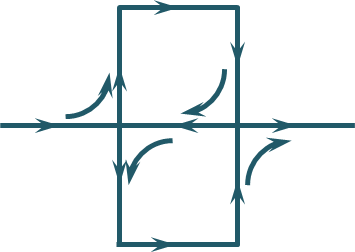
\includegraphics[width=.55\linewidth]{images/peano}
\end{center}


\end{multicols}



